\documentclass[11pt]{article}
\usepackage{graphicx}
\graphicspath{/Users/georgeadams/Dropbox/005_ITP_projects/003 TPO/R commands for TPO/}
\usepackage[utf8]{inputenc}

\title{}
\author{George Adams .... Nichola Cooper}
\date{July 2018}

\begin{document}

\maketitle

\paragraph{Introduction:} Thrombopoietin (TPO) is the main regulator of platelet production and TPO-mimetics are increasingly being used as treatment in immune thrombocytopenia in which TPO levels appear to be inappropraitely low, the reasons for which are not fully understood. The prevailing hypothesis is that TPO binds to platelets via high-affinity receptors on their surface and thus becomes sequestered out of the circulation. The lower-than-expected TPO levels in ITP reflect a higher turnover of platelets. To test this hypothesis we measured TPO levels in a 75 patients with ITP and other thrombocytopenic conditions with the aim of investigating how TPO levels change with platelet counts. For those patient ITP (We used a bayesian statistical regression model to analyse the association as this allows us to infer TPO concentration over a range of different platelet counts and is generally more accurate with smaller sample sizes than classical gaussian regression models.


\paragraph{Methods:} 75 thrombocytopenic patients had blood samples taken between May to November 2014 in an outpatients setting. 67 patients had a diagnosis of ITP and 8 patients with a bone marrow-failure syndrome (4 aplastic anaemia, 3 post- BMT, 1 MDS). In total 130 samples were sent for TPO plasma levels with the majority of patients having duplicate samples. For the TPO analysis, blood samples were collected in sodium citrate tubes, double spun to remove platelet fractions and then stored at -80°C within four hours of collection. Patients also had a full blood count measured at the time of collection. TPO levels measurements perfomed by quantitive sandwich enzyme immunoassay technique. For analysis, a bayesian regression model was used of (log-normalised) platelet count regressed against (log-normalised) TPO; $log(TPO) = alpha + beta*log(platelet)$. We used uninformative gaussian priors (mean 0, standard deviation 10) for the model. Using this model we predicted posteriors distributions for a range of different platelet counts (1, 10 & 150) to determine estimated TPO distributions.

\paragraph{Results:} Of the 130 samples collected, we excluded 30 which failed to show any TPO result. We had positive repeat samples on many of these patients which indicated these zero values where due to laboratory assay failures rather than true absence of TPO. TPO levels concentrations ranged from 15 to 4572.5pg/mL (normal range for health individual ~ 80pg/ml) and platelet counts ranged from 4 to 452 x$10^9/L$. In those with ITP (n=121) the TPO range was between 14-829.3pg/ml. We predicted TPO distributions for platelet counts; 1,3,5, 7 10, 20 and 200 for patients with ITP. Figure 1 (A.) shows the plotted distributions for both the ITP and non-ITP patients. In those patients without ITP the maximium a posteriori (MAP) estimation was  The We plotted \textsubscript{log}TPO levels against platelet counts.  The Bayesian regression model found that for the patients with ITP TPO levels increased in a linear fashion as platelet counts fell from 10 to 1. However, for platelet counts \geqslant 10 the TPO levels remained approximately the same (MAP estimate approximately 210, bayesian interval 156 to 278). This was also found in our cubic spline regression model (Figure 1,B) which found a flattening of TPO levels as platelet counts rose. For those patients with BMF/non-ITP causes of thrombocytopenia, their TPO were considerably higher at lower platelet counts that the ITP patients, which is consistent with the literature.  In the non-ITP cases the distribution predicted TPO concentrations in the non-ITP cases could be very wide even with higher platelet counts. We modelled the relationship between $Log$TPO concentrations and platelet count using a smoothing spline regression model. This also found in patients with ITP that after a platelet count of approximately 10 the TPO concentration in the blood stabilised. The regression smoothing spline model however indicated that for the the bone marrow failure syndromes however the TPO levels fell significantly. This is consistent with the bayesian model which showed a potentially very wide TPO distribution at higher platelet counts. This may also reflects the heterogeneity of this in terms of bone marrow pathology.
\paragraph{Conclusions:}


\begin{center}
 \begin{tabular}{||c c c c c||}
 \hline
 Non-ITP   & platelet count & MAP & LL & UL \\ [0.5ex]
 \hline\hline
 Platelet count & 1 & 80.64 & 52 & 122 \\
 \hline
 Patelet count & 10 & 62 & 41 & 93 \\
 \hline
 Platelet count & 20 & 73 & 14  & 333 \\
 \hline
 Platelet count & 200 & INF & 0 & INF \\
 \hline\hline
  ITP   & platelet count & MAP & LL & UL    \\
\hline\hline
 Platelet count & 1 & 407 & 320  & 518 \\
 \hline
 Patelet count & 10 & 214 & 164 & 281 \\
 \hline
 Platelet count & 20 & 208 & 156 & 278 \\
 \hline
 Platelet count & 200 & 208 & 156 & 278 \\ [1ex]
 \hline
\end{tabular}
\end{center}

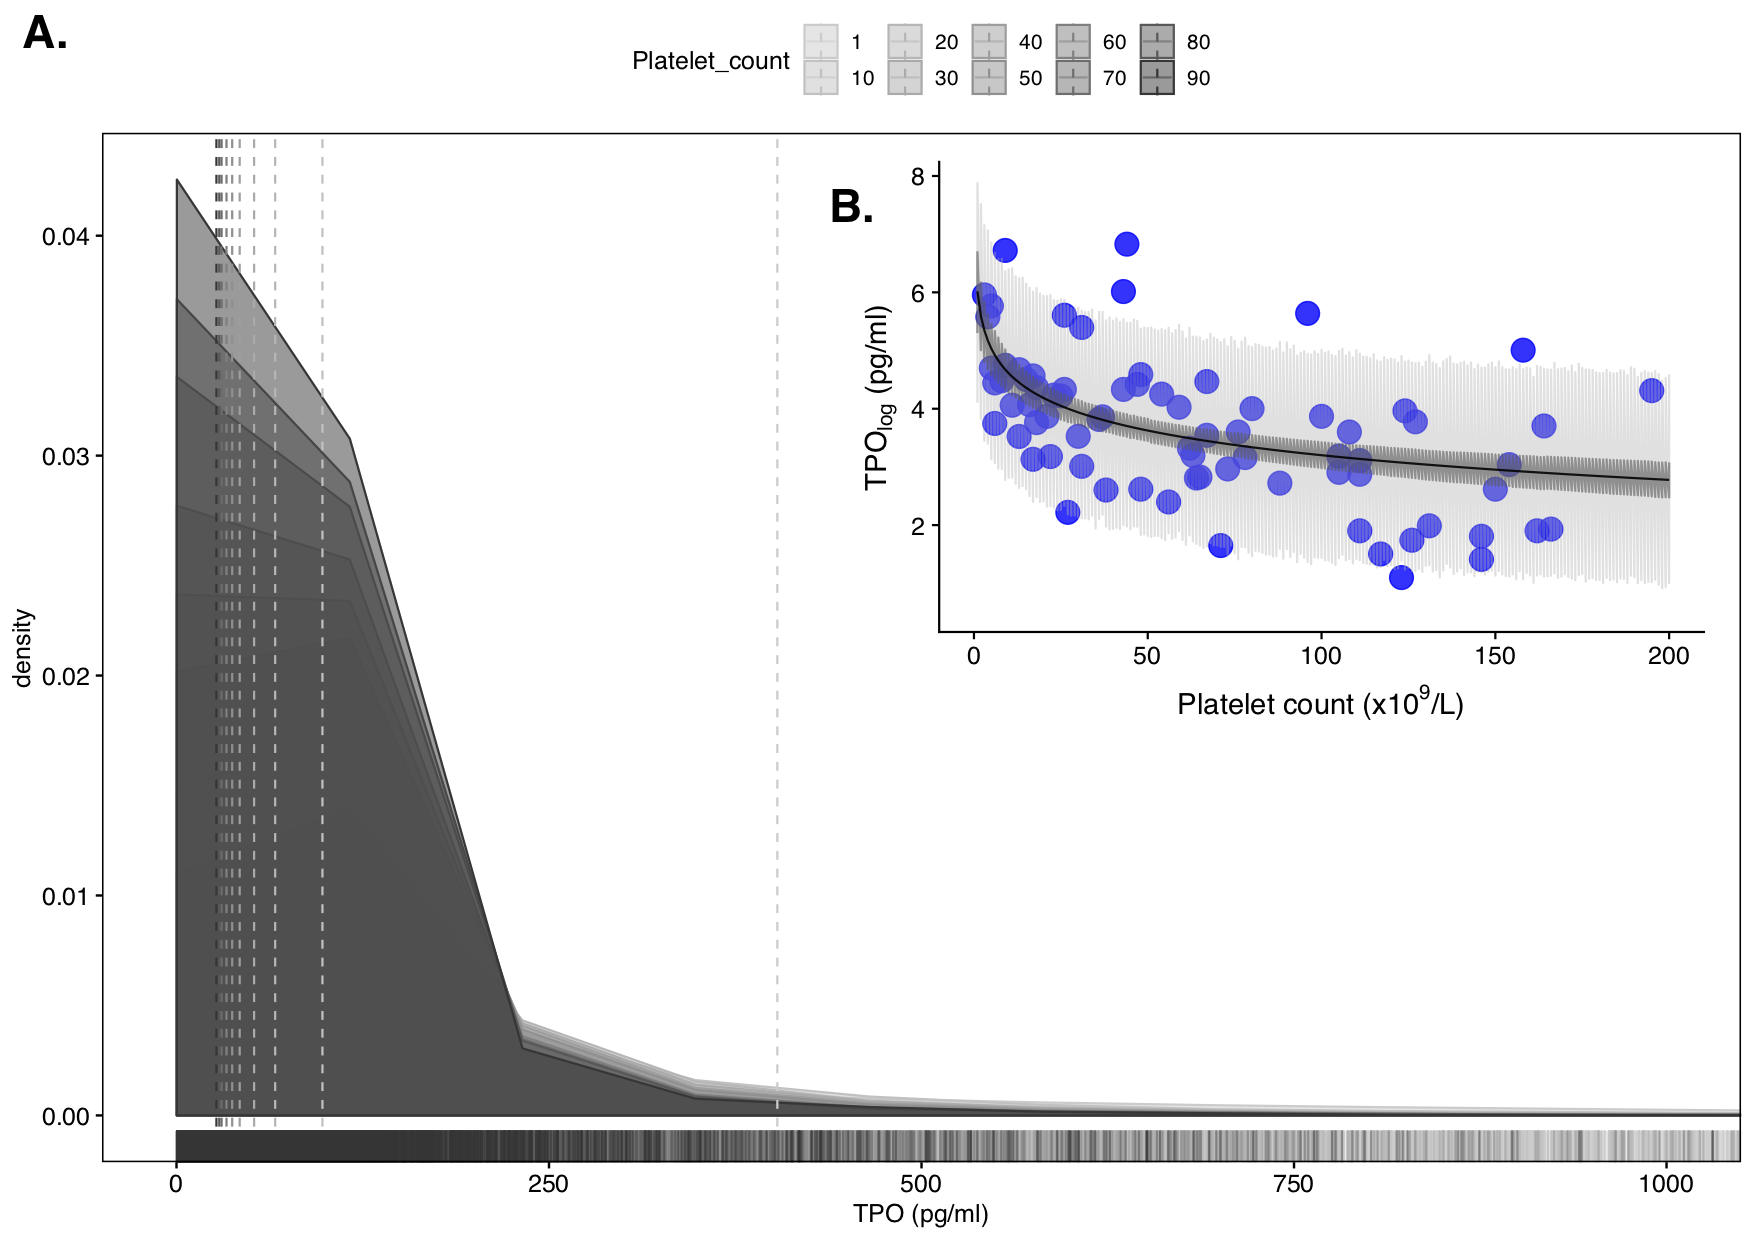
\includegraphics[FIGURE 1: A. Shows predicted TPO distributions for at different platelet counts ranging from 10 to 90. Dashed vertical lines represent median values for each distribution. B. LogTPO levels versus platelet counts showing individual patient results and the predicted non-linear assocaition produced by model. Darker shaded area is the 90\% bayesian confidence interval and the lighter shaded area around curve shows total predicted distribution width]{ABSTRACT_v1_graph1.png}

\paragraph{}
\textbf{Total characters: 3800}


\end{document}
